% Template for a Computer Science Tripos Part II project dissertation
\documentclass[12pt,a4paper,twoside,openright]{report}
\usepackage[pdfborder={0 0 0}]{hyperref} % turns references into hyperlinks
\usepackage[margin=25mm]{geometry} % adjusts page layout
\usepackage{graphicx} % allows inclusion of PDF, PNG and JPG images
\usepackage{verbatim}
\usepackage{docmute} % only needed to allow inclusion of proposal.tex
\raggedbottom % try to avoid widows and orphans
\sloppy
\clubpenalty1000%
\widowpenalty1000%
\renewcommand{\baselinestretch}{1.1} % adjust line spacing to make
% more readable
\begin{document}
\bibliographystyle{plain}
%%%%%%%%%%%%%%%%%%%%%%%%%%%%%%%%%%%%%%%%%%%%%%%%%%%%%%%%%%%%%%%%%%%%%%%%
% Title
\pagestyle{empty}
\rightline{\LARGE \textbf{Martin Richards}}
\vspace*{60mm}
\begin{center}
\Huge
\textbf{How to write a dissertation in \LaTeX} \\[5mm]
Computer Science Tripos -- Part II \\[5mm]
St John's College \\[5mm]
\today % today's date
\end{center}
%%%%%%%%%%%%%%%%%%%%%%%%%%%%%%%%%%%%%%%%%%%%%%%%%%%%%%%%%%%%%%%%%%%%%%%%%%%%%%
% Proforma, table of contents and list of figures
\pagestyle{plain}
\chapter*{Proforma}
{\large
\begin{tabular}{ll}
Name: & \bf Martin Richards \\
College: & \bf St John's College \\
Project Title: & \bf How to write a dissertation in \LaTeX \\
Examination: & \bf Computer Science Tripos -- Part II, July 2001 \\
Word Count: & \bf 1587\footnotemark[1]
(well less than the 12000 limit) \\
Project Originator: & Dr M.~Richards \\
Supervisor: & Dr Markus Kuhn \\
\end{tabular}
}
\footnotetext[1]{This word count was computed
by \texttt{detex diss.tex | tr -cd '0-9A-Za-z $\tt\backslash$n' | wc -w}
}
\stepcounter{footnote}
\section*{Original Aims of the Project}
To write a demonstration dissertation\footnote{A normal footnote without the
complication of being in a table.} using \LaTeX\ to save
student's time when writing their own dissertations. The dissertation
should illustrate how to use the more common \LaTeX\ constructs. It
should include pictures and diagrams to show how these can be
incorporated into the dissertation. It should contain the entire
\LaTeX\ source of the dissertation and the makefile. It should
explain how to construct an MSDOS disk of the dissertation in
Postscript format that can be used by the book shop for printing, and,
finally, it should have the prescribed layout and format of a diploma
dissertation.
\section*{Work Completed}
All that has been completed appears in this dissertation.
\section*{Special Difficulties}
Learning how to incorporate encapulated postscript into a \LaTeX\
document on both Ubuntu Linux and OS X.
\newpage
\section*{Declaration}
I, [Name] of [College], being a candidate for Part II of the Computer
Science Tripos [or the Diploma in Computer Science], hereby declare
that this dissertation and the work described in it are my own work,
unaided except as may be specified below, and that the dissertation
does not contain material that has already been used to any substantial
extent for a comparable purpose.
\bigskip
\leftline{Signed [signature]}
\medskip
\leftline{Date [date]}
\tableofcontents
\listoffigures
\newpage
\section*{Acknowledgements}
This document owes much to an earlier version written by Simon Moore
\cite{Moore95}. His help, encouragement and advice was greatly
appreciated.
%%%%%%%%%%%%%%%%%%%%%%%%%%%%%%%%%%%%%%%%%%%%%%%%%%%%%%%%%%%%%%%%%%%%%%%
% now for the chapters
\pagestyle{headings}
\chapter{Introduction}
\section{Overview of the files}
This document consists of the following files:
\begin{itemize}
\item \texttt{makefile} --- The makefile for the dissertation and
Project Proposal
\item \texttt{diss.tex} --- The dissertation
\item \texttt{proposal.tex} --- The project proposal
\item \texttt{figs} -- A directory containing diagrams and pictures
\item \texttt{refs.bib} --- The bibliography database
\end{itemize}
\section{Building the document}
This document was produced using \LaTeXe which is based upon
\LaTeX\cite{Lamport86}. To build the document you first need to
generate \texttt{diss.aux} which, amongst other things, contains the
references used. This if done by executing the command:
\texttt{pdflatex diss}
\noindent
Then the bibliography can be generated from \texttt{refs.bib} using:
\texttt{bibtex diss}
\noindent
Finally, to ensure all the page numbering is correct run \texttt{pdflatex}
on \texttt{diss.tex} until the \texttt{.aux} files do not change. This
usually takes 2 more runs.
\subsection{The makefile}
To simplify the calls to \texttt{pdflatex} and \texttt{bibtex},
a makefile has been provided, see Appendix~\ref{makefile}.
It provides the following facilities:
\begin{description}
\item\texttt{make} \\
Display help information.
\item\texttt{make proposal.pdf} \\
Format the proposal document as a PDF.
\item\texttt{make view-proposal} \\
Run \texttt{make proposal.pdf} and then display it with a Linux PDF viewer
(preferably ''okular'', if that is not available fall back to ''evince'').
\item\texttt{make diss.pdf} \\
Format the dissertation document as a PDF.
\item\texttt{make count} \\
Display an estimate of the word count.
\item\texttt{make all} \\
Construct \texttt{proposal.pdf} and \texttt{diss.pdf}.
\item\texttt{make pub} \\ Make \texttt{diss.pdf}
and place it in my \texttt{public\_html} directory.
\item\texttt{make clean} \\ Delete all intermediate files except the
source files and the resulting PDFs. All these deleted files can
be reconstructed by typing \texttt{make all}.
\end{description}
\section{Counting words}
An approximate word count of the body of the dissertation may be
obtained using:
\texttt{wc diss.tex}
\noindent
Alternatively, try something like:
\verb/detex diss.tex | tr -cd '0-9A-Z a-z\n' | wc -w/
\chapter{Preparation}
This chapter is empty!
\chapter{Implementation}
\section{Verbatim text}
Verbatim text can be included using \verb|\begin{verbatim}| and
\verb|\end{verbatim}|. I normally use a slightly smaller font and
often squeeze the lines a little closer together, as in:
{\renewcommand{\baselinestretch}{0.8}\small
\begin{verbatim}
GET "libhdr"
GLOBAL { count:200; all }
LET try(ld, row, rd) BE TEST row=all
THEN count := count + 1
ELSE { LET poss = all & ~(ld | row | rd)
UNTIL poss=0 DO
{ LET p = poss & -poss
poss := poss - p
try(ld+p << 1, row+p, rd+p >> 1)
}
}
LET start() = VALOF
{ all := 1
FOR i = 1 TO 12 DO
{ count := 0
try(0, 0, 0)
writef("Number of solutions to %i2-queens is %i5*n", i, count)
all := 2*all + 1
}
RESULTIS 0
}
\end{verbatim}
}
\section{Tables}
\begin{samepage}
Here is a simple example\footnote{A footnote} of a table.
\begin{center}
\begin{tabular}{l|c|r}
Left & Centred & Right \\
Justified & & Justified \\[3mm]
%\hline\\%[-2mm]
First & A & XXX \\
Second & AA & XX \\
Last & AAA & X \\
\end{tabular}
\end{center}
\noindent
There is another example table in the proforma.
\end{samepage}
\section{Simple diagrams}
Simple diagrams can be written directly in \LaTeX. For example, see
figure~\ref{latexpic1} on page~\pageref{latexpic1} and see
figure~\ref{latexpic2} on page~\pageref{latexpic2}.
\begin{figure}
\setlength{\unitlength}{1mm}
\begin{center}
\begin{picture}(125,100)
\put(0,80){\framebox(50,10){AAA}}
\put(0,60){\framebox(50,10){BBB}}
\put(0,40){\framebox(50,10){CCC}}
\put(0,20){\framebox(50,10){DDD}}
\put(0,00){\framebox(50,10){EEE}}
\put(75,80){\framebox(50,10){XXX}}
\put(75,60){\framebox(50,10){YYY}}
\put(75,40){\framebox(50,10){ZZZ}}
\put(25,80){\vector(0,-1){10}}
\put(25,60){\vector(0,-1){10}}
\put(25,50){\vector(0,1){10}}
\put(25,40){\vector(0,-1){10}}
\put(25,20){\vector(0,-1){10}}
\put(100,80){\vector(0,-1){10}}
\put(100,70){\vector(0,1){10}}
\put(100,60){\vector(0,-1){10}}
\put(100,50){\vector(0,1){10}}
\put(50,65){\vector(1,0){25}}
\put(75,65){\vector(-1,0){25}}
\end{picture}
\end{center}
\caption{A picture composed of boxes and vectors.}
\label{latexpic1}
\end{figure}
\begin{figure}
\setlength{\unitlength}{1mm}
\begin{center}
\begin{picture}(100,70)
\put(47,65){\circle{10}}
\put(45,64){abc}
\put(37,45){\circle{10}}
\put(37,51){\line(1,1){7}}
\put(35,44){def}
\put(57,25){\circle{10}}
\put(57,31){\line(-1,3){9}}
\put(57,31){\line(-3,2){15}}
\put(55,24){ghi}
\put(32,0){\framebox(10,10){A}}
\put(52,0){\framebox(10,10){B}}
\put(37,12){\line(0,1){26}}
\put(37,12){\line(2,1){15}}
\put(57,12){\line(0,2){6}}
\end{picture}
\end{center}
\caption{A diagram composed of circles, lines and boxes.}
\label{latexpic2}
\end{figure}
\section{Adding more complicated graphics}
The use of \LaTeX\ format can be tedious and it is often better to use
encapsulated postscript (EPS) or PDF to represent complicated graphics.
Figure~\ref{epsfig} and~\ref{xfig} on page \pageref{xfig} are
examples. The second figure was drawn using \texttt{xfig} and exported in
{\tt.eps} format. This is my recommended way of drawing all diagrams.
\begin{figure}[tbh]
\centerline{\includegraphics{figs/cuarms.pdf}}
\caption{Example figure using encapsulated postscript}
\label{epsfig}
\end{figure}
\begin{figure}[tbh]
\vspace{4in}
\caption{Example figure where a picture can be pasted in}
\label{pastedfig}
\end{figure}
\begin{figure}[tbh]
\centerline{\includegraphics{figs/diagram.pdf}}
\caption{Example diagram drawn using \texttt{xfig}}
\label{xfig}
\end{figure}
\chapter{Evaluation}
\section{Printing and binding}
Use a ''duplex'' laser printer that can print on both sides to print
two copies of your dissertation. Then bind them, for example using the
comb binder in the Computer Laboratory Library.
\section{Further information}
See the Unix Tools notes at
\url{http://www.cl.cam.ac.uk/teaching/current-1/UnixTools/materials.html}
\chapter{Conclusion}
I hope that this rough guide to writing a dissertation is \LaTeX\ has
been helpful and saved you time.
%%%%%%%%%%%%%%%%%%%%%%%%%%%%%%%%%%%%%%%%%%%%%%%%%%%%%%%%%%%%%%%%%%%%%
% the bibliography
\addcontentsline{toc}{chapter}{Bibliography}
\bibliography{refs}
%%%%%%%%%%%%%%%%%%%%%%%%%%%%%%%%%%%%%%%%%%%%%%%%%%%%%%%%%%%%%%%%%%%%%
% the appendices
\appendix
\chapter{Latex source}
\section{diss.tex}
{\scriptsize\verbatiminput{diss.tex}}
\section{proposal.tex}
{\scriptsize\verbatiminput{proposal.tex}}
\chapter{Makefile}
\section{makefile}\label{makefile}
{\scriptsize\verbatiminput{makefile.txt}}
\section{refs.bib}
{\scriptsize\verbatiminput{refs.bib}}
\chapter{Project Proposal}
\documentclass[12pt]{article}
\usepackage{graphicx, indentfirst, tikz, gensymb, url} % Required for inserting images
\usepackage[load-configurations = abbreviations]{siunitx}
\def\checkmark{\tikz\fill[scale=0.4](0,.35) -- (.25,0) -- (1,.7) -- (.25,.15) -- cycle;} 

\title{Building a Physics Engine From Scratch}
\author{js2657}
\date{Oct 2023}

\begin{document}


Proposal Draft V2

Building a Physics Engine From Scratch

Supervisor: Joe G March

UTO: Rafal Mantiuk

TODO:

0: Typeset \checkmark

1: Add references \checkmark

2: Grammar check \checkmark

3: Expand on extensions \checkmark

4: Add Evaluation section \checkmark

5: Add tables and images \checkmark

Issues:

0: One main issue is, how should I deal with success criteria?
On the one hand, I agree with Richard's feedback that saying something too explicit is dangerous, 
and sometimes discouraging due to being unrealistic to compare such a project with real-life huge projects.
On the other hand, many people seem to have expected some definitive success criteria to be stated.
This is showed through the checker feedback, as well as many past project proposals where there are many examples of 
"I will achieve significantly better results than X"

1: Is the current evaluation perhaps a bit too specific?

Checker feedback:

you need to put the actual references, as they would help us understand the context of your project.
\checkmark

As stated in phase I, you need to identify a UTO/supervisor who would help you shape the proposal
\checkmark

Give that there are a lot of open source physics engines, I am not convinced that developing your own will address their shortcoming that the computations are done under the hood. Need to have a different motivation
\checkmark

It is good that you will be comparing against existing engines. What will you be looking for in this comparison? What will be the success criteria for your project? You need to define these ASAP.
[Refer to issue 0]

Also pick one or two extensions and expand on them to ensure that we have a good plan for the project.\checkmark

DoS feedback:

My main feedback on this is that you need to have some evaluation in your core. 
You should decide what that is and specify it explicitly.
A bit more specifically I mean.
So would give some examples of how you intend to quantitatively compare your engine to others.
\checkmark

As a point of style I'd use 'heuristics' instead of 'hacky methods' 
\checkmark

And I would recommend explicitly stating that you're going to model velocity and angular velocity of rigid bodies in your core. 
(I know you say it in the description; but would include it again for good measure)
\checkmark

I think the references are missing too
\checkmark

Also fix the latex section numbers to avoid the '0.n' thing 
\checkmark


\section{Introduction}

Physics Engine, a term frequently used in video game industry and science research, 
is a tool that simulates physical phenomena using a computer.
The first computer, ENIAC, at one point used a physics engine to help design military weapons\cite{rojas2002first}.
At the core of physics engine, semi-realistic results are obtained through a combination of 
computation-efficient numerical approximations, 
careful modelling of the objects, 
and sometimes clever hacks that enable the engine to just make the cut.

There are some common terminologies in physics engines.
\begin{itemize}
\item \textbf{Rigid body} is an individual object that will be simulated in the engine.
A rigid body is an object that does not distort or bend, as opposed to soft body or fluid, 
which gives rigid bodies the benefit of simplicity.
A typical physics engine needs to keep track of its mass, position, orientation, linear velocity, angular velocity and impulse.
\item \textbf{Collider} is a part of a rigid body.
Complex rigid bodies tend to get separated into simple, convex colliders like spheres and boxes in the pipeline.
\item \textbf{Collision detection} and \textbf{Collision resolution} are components of the engine which handle the interaction between colliders.
Commonly physics engine continuously advances the time by a small fraction of a second, moving the objects according to their speed.
After each position update, Collision detection will kick in and detect if a pair of colliders will intersect.
If so, Collision resolution will decide whether and how they will get bounced and separated apart, 
updating their velocities accordingly.
\end{itemize}

Many open-source physics engines are available online, including PhysX\cite{physx}, 
Box2D\cite{box2d} and Bullet\cite{bullet}.
However, the most common way a physics engine is presented is as a big, mysterious library 
where all the computation is done under dozens of dependencies and documentation.
As a result, adding a simple feature could take a lot of effort of plowing through documentation and files.
I want to build my own physics engine, 
which gives me the flexibility to add whatever I want because I would know exactly how it works.

\section{Description}

My project aims to build a 3D real-time physics engine from scratch that implements basic modules, 
without making use of any currently available physics engine.
My focus will be to realise the visual effects rather than being extremely accurate or efficient,
considering the limited time, my available hardware resources, and the ease of experiments and showcases.
This is also why I chose to build a real-time physics engine over a high-precision one.
In addition, this project will also provide a basic framework that is easy to extend upon in the future, if necessary.
Overall, this project will be a great opportunity for me to learn more about physics and programming.

Here is a list of the basic core modules I plan to implement:
\begin{itemize}
\item Object modelling: Create data structures for recording attributes of rigid bodies and design interfaces for applying forces and adding colliders.
Typical physical attributes of rigid bodies include mass, position, orientation, linear velocity, angular velocity, and impulse.
\item Collision detection: Adopt many algorithms to decide if collisions happen.
\item Bounce: Part of Collision resolution where some maths are used to find the approximated results of a bounce.
\item Friction: Part of Collision resolution where vast assumptions are used to simulate real-life friction.
\item Stability: Part of Collision resolution where some heuristics are used to prevent certain visual artefacts.
For example, if two objects are stacked together, the upper one should not be bouncing up and down constantly.
\end{itemize}

The project could then be evaluated by comparisons using simple experiments against existing popular physics engines.
More on this in the Evaluation section.

Extension modules I plan to look at include:
\begin{itemize}
\item Fluid simulation:

Fluid simulation involves approximations to fluid equations, 
and can have different levels of complexity depending on the topic.
For example, 
the simulation of buoyant force of hard objects submerged in water will be simpler than 
the simulation of the flow of the fluid.
I will try my best to cover as much in fluid simulation as I can.

\item Real-time rendering:

For the sake of showcasing, I might be using existing rendering libraries like Blender\cite{blender}, 
but it is certainly better to not rely on them.

\item Performance evaluation

I will give different implementations for CPU and GPU, 
which will then allow me to draw comparisons about their contributions to performance.

\item Soft-body simulation

Unlike rigid bodies, the shape of objects can change to a certain degree.
Therefore, it is much harder to model them and deal with collisions.
I will need to do research and choose what to implement. 

\end{itemize}

\section{Evaluation}

Evaluation of physics engines can be quite challenging, 
especially when quantitative analysis is preferred.
Little work has been done in this area as of now, 
likely due to the complexity, systematic bias, and the lack of needs.

The evaluation of this project is split into three parts: Benchmark selection, Core functionality, and Performance evaluation.

\subsection{Benchmark selection}

Since the functionality evaluations will be largely comparison-based,
I will be choosing at least three open-source physics engines that support similar features to compare against.
The following engines have been found as possible candidates:

\begin{table}[h]
    \centering
    \makebox[\linewidth]{
    \begin{tabular}
    {|c|c|}
    \hline 
    Physics engine                                & Website                                                         \\
    \hline 
    Advanced Simulation Library                   & asl.org.il                                           \\
    Bullet                                        & pybullet.org                                           \\
    Newton Game Dynamics                          & newtondynamics.com/forum/newton.php                      \\
    Open Dynamics Engine                          & www.ode.org                                            \\
    PAL              & www.adrianboeing.com/pal                                \\
    PhysX                                         & www.nvidia.com/en-gb/geforce/technologies/physx        \\
    Project Chrono~                               & projectchrono.org                                      \\
    Siconos                                       & nonsmooth.gricad-pages.univ-grenoble-alpes.fr/siconos  \\
    SOFA & www.sofa-framework.org                                 \\
    Tokamak physics engine                        & github.com/isegal/TokamakPhysics                        \\
    \hline
    \end{tabular}
    }
\end{table}

I plan to further narrow them down by testing if they work in my environment, 
if they have sufficient documentation, 
and if they support the features I am going to compare on.

\subsection{Core functionality}

The functionality will be evaluated through a series of small runtime tests.
The tests are similar to the ones that already existed\cite{seugling2006evaluation}.
Please note that they are preliminary and might be adjusted for clearer visuals.

\subsubsection{Bounce test}

To test whether the engines could handle object collisions, I measure if the momentum and energy are preserved.

Two identical spheres will be placed in a world with no gravity. 
Sphere A, the one on the left, is located at $(0, 0, 0)$, and is moving along the $+$x direction with a velocity of $\SI{1}{\m\per\s}$.
Sphere B, the one on the right, is located at $(\SI{10}{\m}, 0, 0)$, and is moving along the $-$x direction with a velocity of $\SI{1}{\m\per\s}$.
Both spheres have a radius of 1m and a mass of $\SI{1}{\kg}$. The restitution will vary between $0$ and $1$.

\begin{center}
    \makebox[\textwidth]{
\includegraphics[width=\textwidth]{img1.png}}
  \end{center}

Theoretically, the sum of momentum vectors should stay at $(0, 0, 0)$, and the total energy at $\SI{1}{\J}$.
The actual sum of momentum and total energy, as simulated by the engine, will be plotted against time.
The less these values vary, the more accurate the simulation is.

\subsubsection{Friction test}

Coulomb's Law describes the friction force with the coefficient of friction, $\mu$, which is a constant property of the surface.
If the friction force is $F_f$, the normal force exerted by the surface is $F_n$, then it holds that

\begin{equation}
F_f \leq \mu \times F_n
\end{equation}

Therefore,

\begin{equation}
\frac{F_f}{F_n} \leq \mu
\end{equation}

A box will be placed on a static inclined plane, whose coefficient $\mu = 0.5$.
The angle the surface is tilted by, theta, will gradually increase from 0 to $\frac{\pi}{2}$
A cube of $\SI{1}{\m} \times \SI{1}{\m} \times \SI{1}{\m}$ will be placed on that plane.
A force of gravity $G = \SI{10}{\N}$ will be applied to the cube.

\begin{center}
    \makebox[\textwidth]{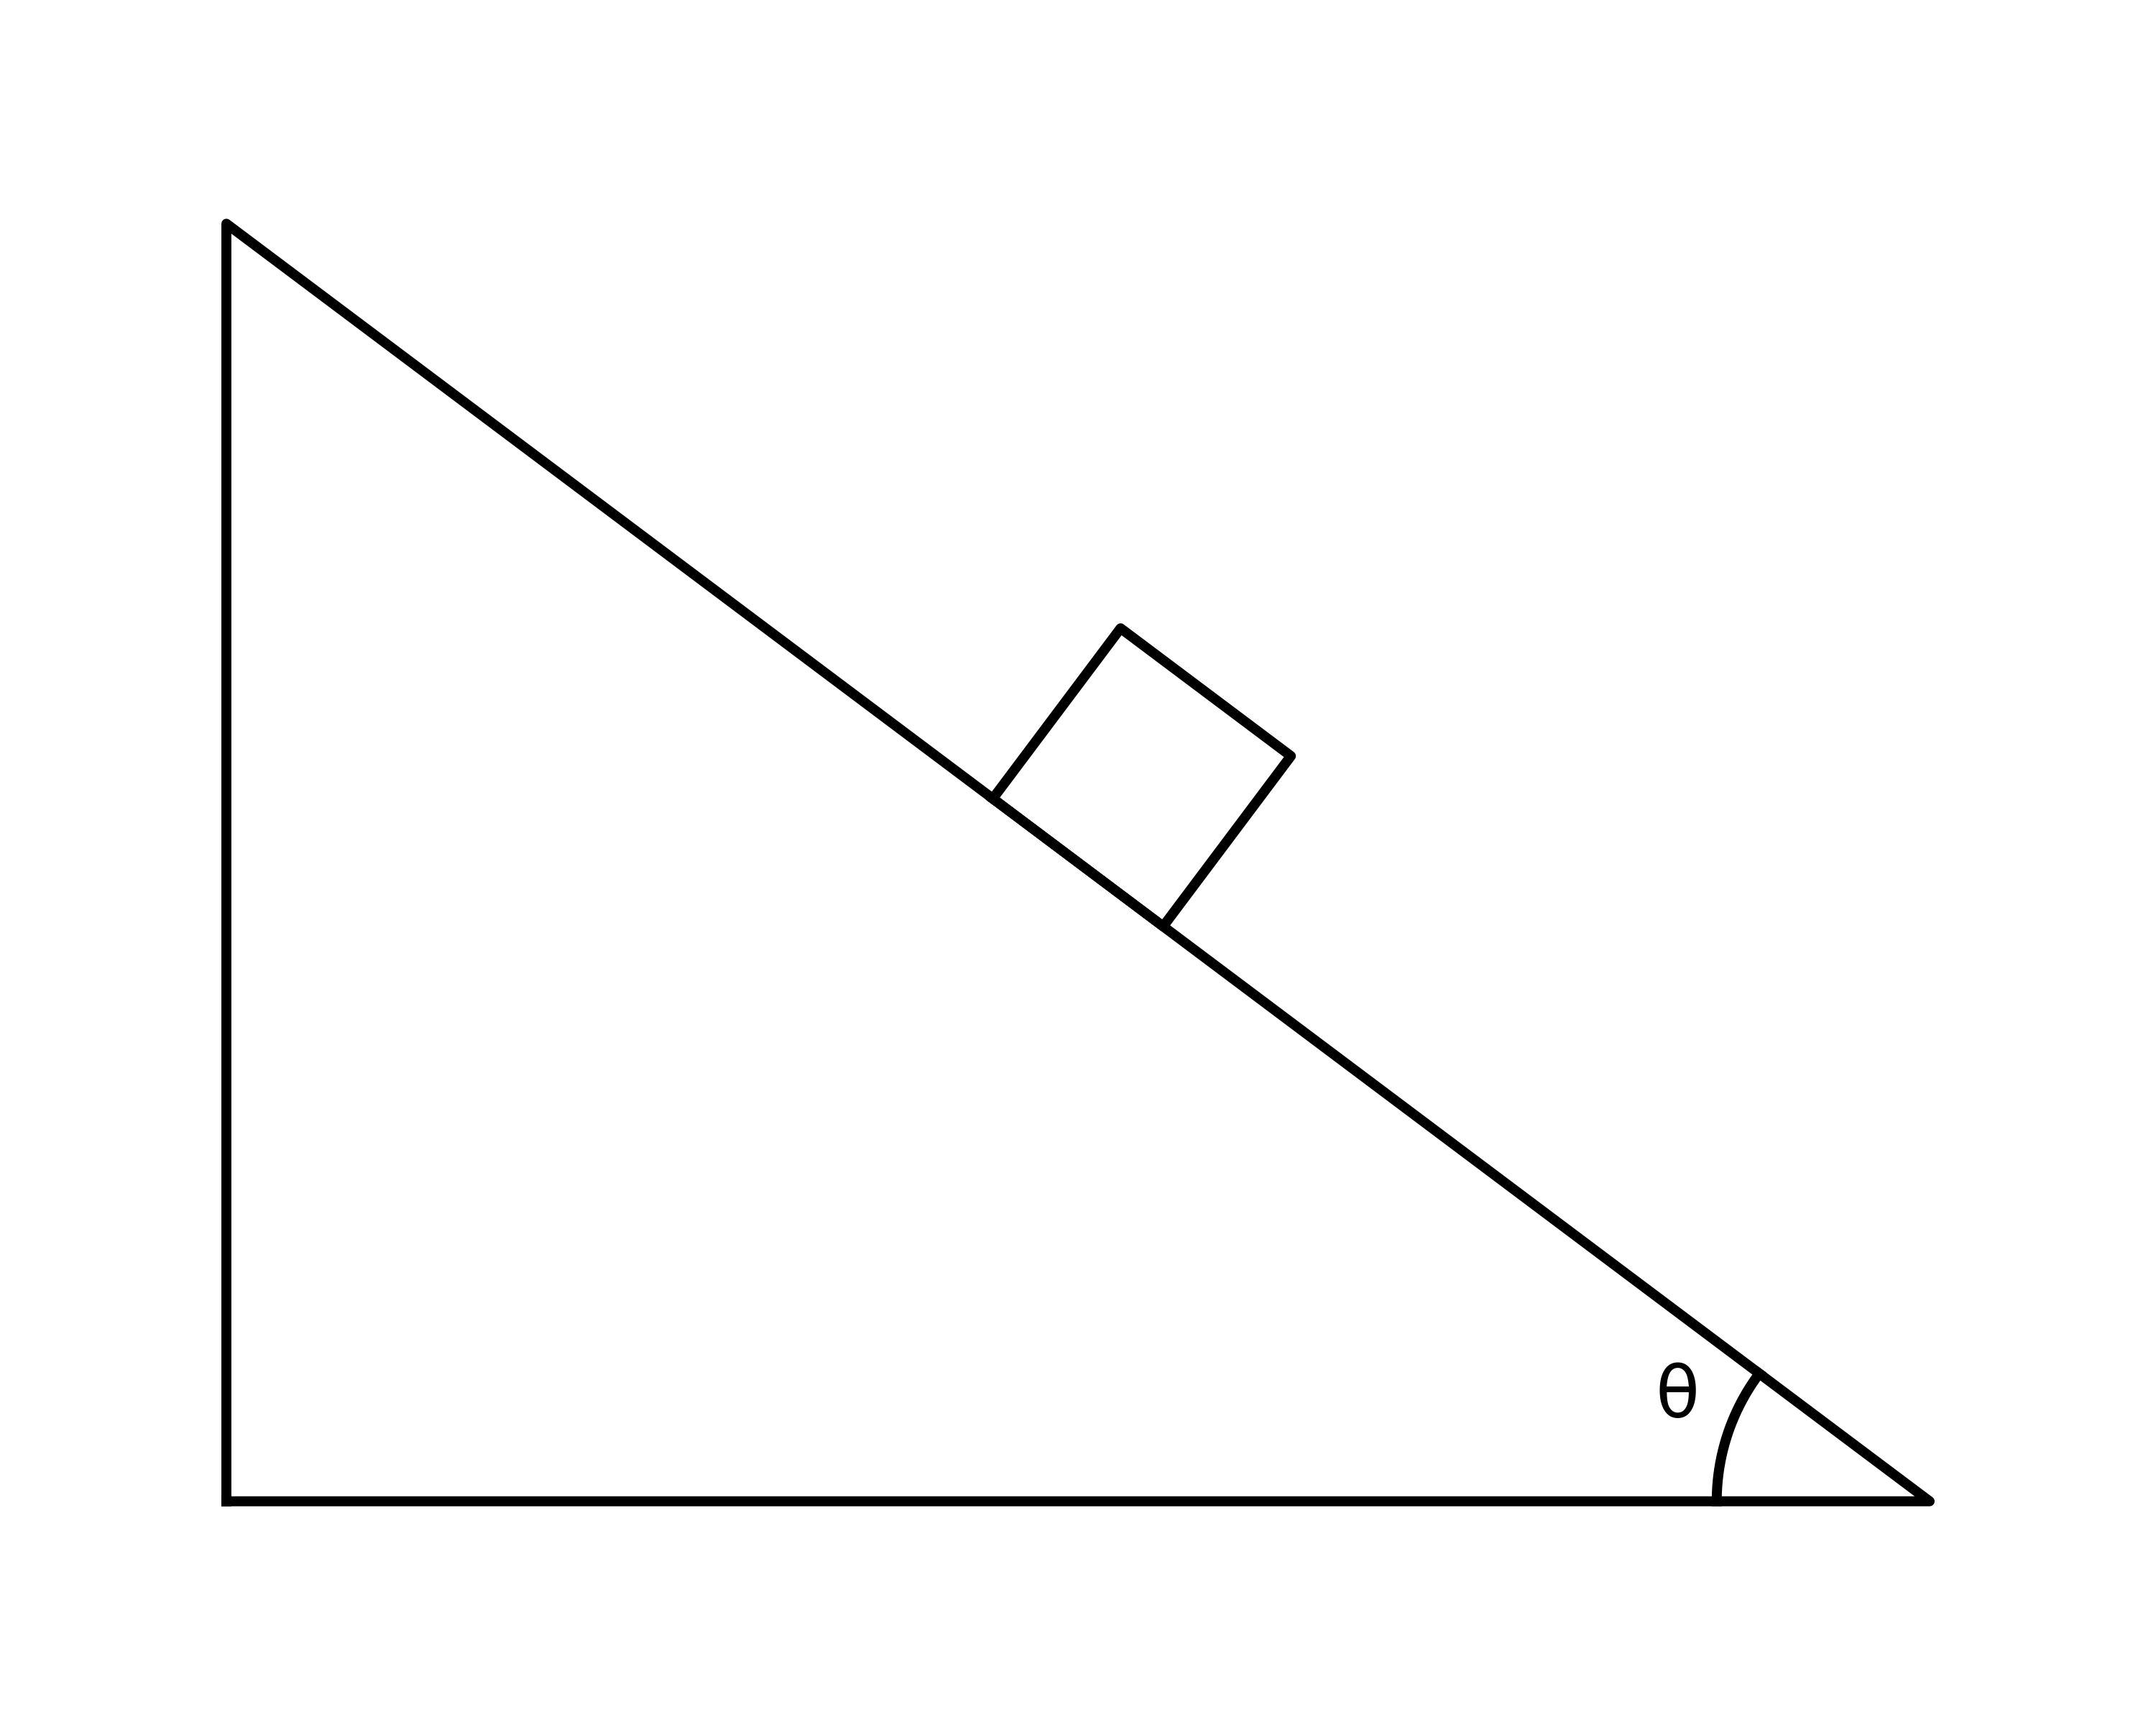
\includegraphics[width=0.5\textwidth]{img2.png}}
  \end{center}

For each angle $\theta$, forces $F_f$ and $F_n$ will be computed as follows.

The normal force is equal to the proportion of gravity perpendicular to the surface:

\begin{equation}
F_n = G \times \cos \theta
\end{equation}

The friction force is calculated using Newton's First Law:

\begin{equation}
F_f = m \times a - G \times \sin \theta
\end{equation}

Now, $\frac{F_f}{F_n}$ will be plotted against the angle theta. According to Coulomb's Law, it should always stay below $\mu = 0.5$

\subsubsection{Pendulum test}

Have a pendulum setup like in the following figure.
A sphere of radius 1m is attached to a fixed point using a bar of radius $\SI{0.001}{\m}$ and length of $\SI{10}{\m}$.
The initial angle between the bar that connects the sphere and an imaginary vertical line through the fixed point is $\theta$.

\begin{center}
    \makebox[\textwidth]{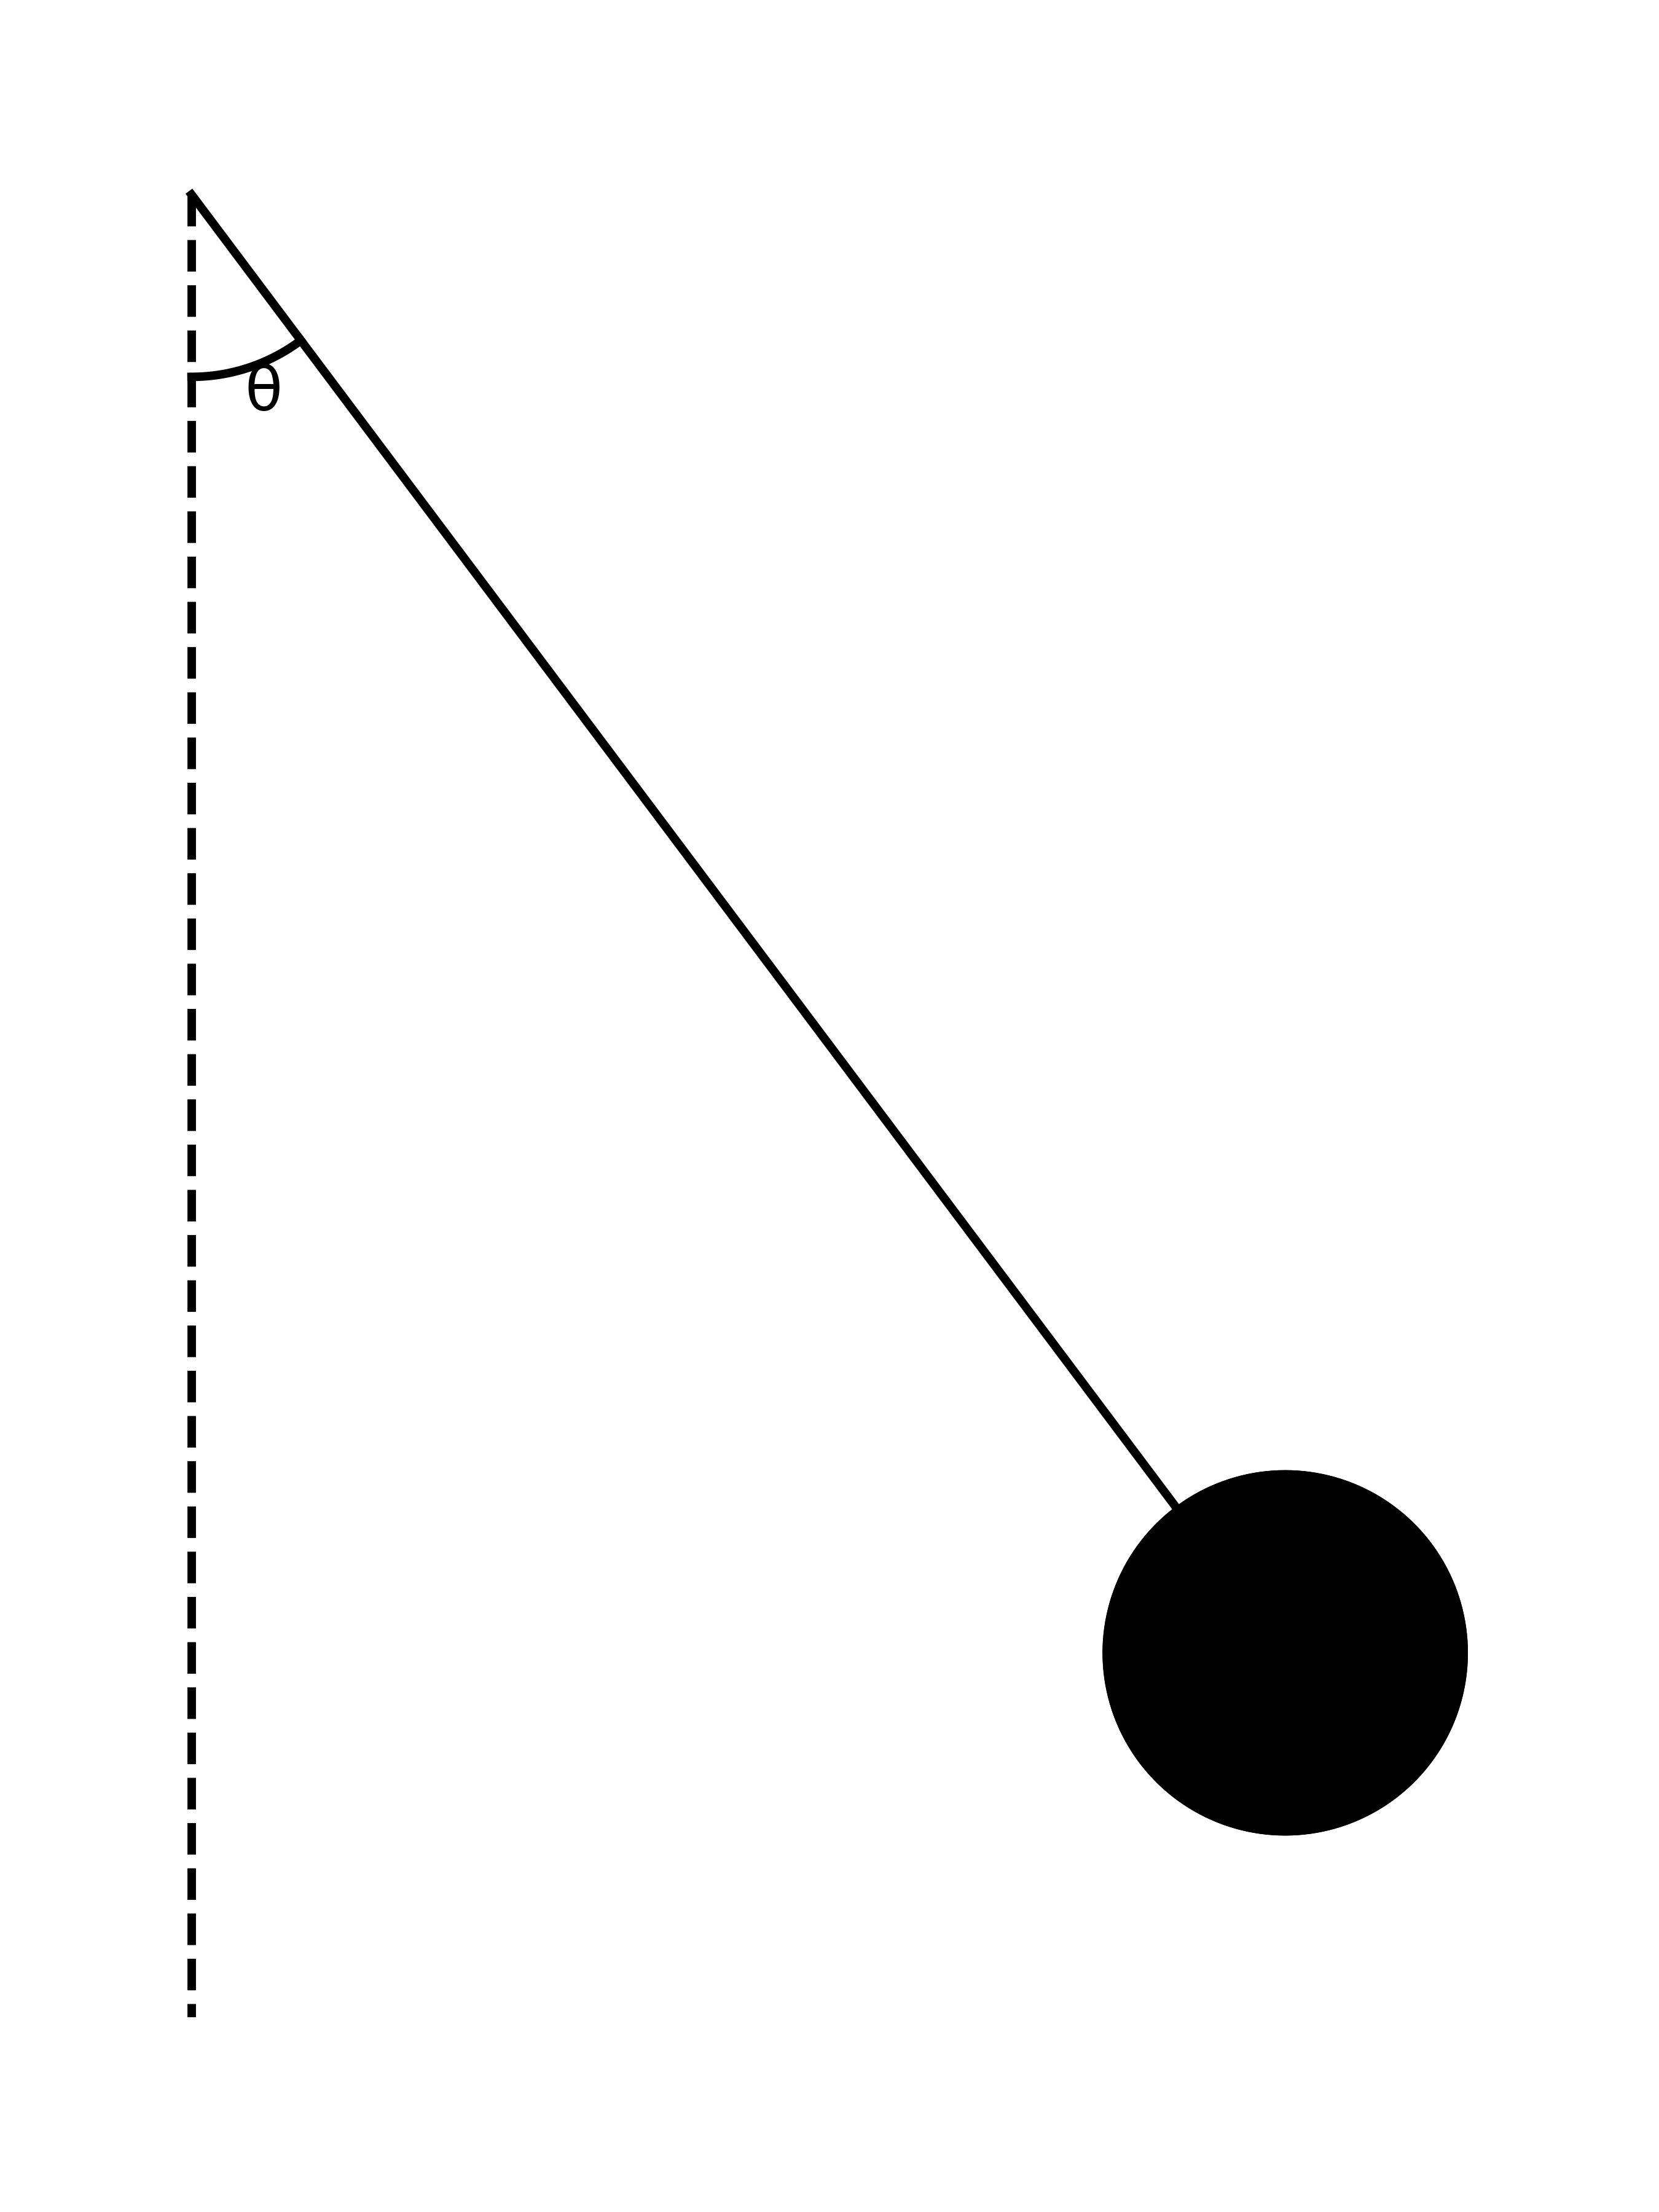
\includegraphics[width=0.3\textwidth]{img3.png}}
  \end{center}

Theta is gradually increased from $5\degree$ to $85\degree$.
For each theta, 
the period of the pendulum is measured by recording the time it takes for the sphere to reach its lowest point $100$ times.

Theoretically, the period of a pendulum is

\begin{equation}
T = 2  \pi \cdot \sqrt{\frac{1}{g}}
\end{equation}

The periods as simulated by the engines will be plotted against the angle theta.

\subsection{Performance evaluation}

This part is considered as an extension. The performance will similarly be measured with a test.

There will be comparisons between my engine and other benchmark engines, as well as between different implementations of my engine.

\subsubsection{Falling test}

a total number of $n$ cubes, all of size $\SI{1}{\m} \times \SI{1}{\m} \times \SI{1}{\m}$, 
are placed at $(0, 0, \SI{2}{\m}), (0, 0, \SI{4}{\m}), \ldots, (0, 0, (n \times 2)\SI{}{\m})$ above a plane of $z = 0$, 
as shown below.
The masses of each cube is chosen uniformly between $\SI{1}{\kg}$ to $\SI{10}{\kg}$, in order to add complexity.

\begin{center}
  \makebox[\textwidth]{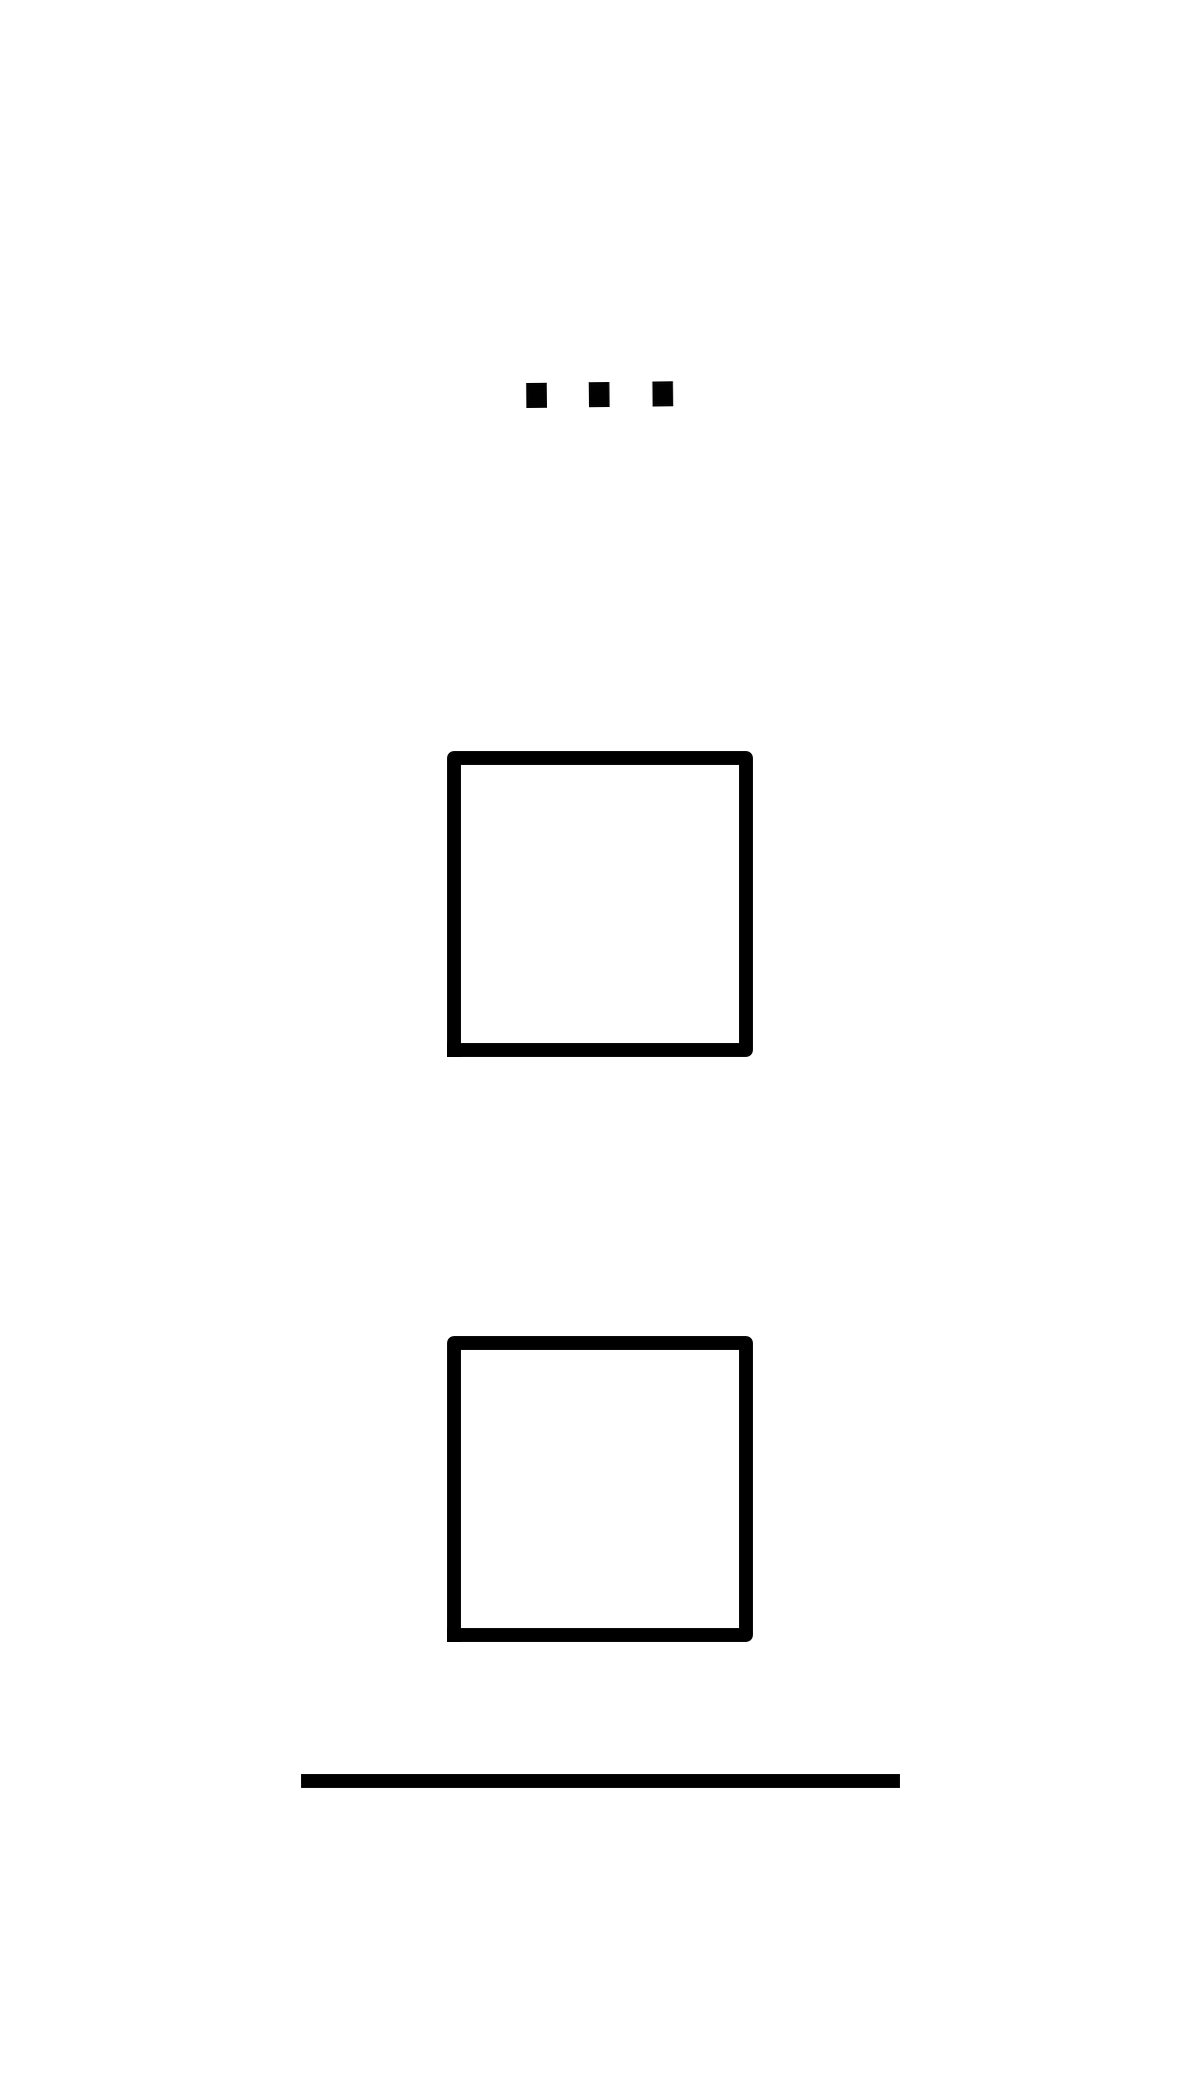
\includegraphics[width=0.3\textwidth]{img4.png}}
\end{center}

The average computational time of a time step is measured and plotted against the number of cubes, $n$.
The average computational time is defined as the average of computational time 
it takes for my machine to simulate the scene in the first $n$ seconds.

\section{Starting Point}

Personally, I have some basic knowledge of programming in C++, having completed a small project using it during my internship.
My graphics knowledge only comes from the two Part IA and IB graphics courses.

Additionally, I have done a bit of research online, 
and am therefore decently confident about the abundance of tutorial resources, 
despite not actually having spent time reading through them.
For example, a full video series about physics engine is available on the Internet\cite{tutorialyt}.
I might also make use of 3D graphics libraries like CUDA\cite{cuda}, but as of now I have no prior working experience with them.

The aforementioned open-source physics engine libraries are also available for me to look into some possible solutions or draw comparisons, 
but I will not be using their simulation code in my project.

\section{Success criteria}

For the core:

\begin{itemize}
\item Implement all basic modules: Object modelling, Collision detection, Bounce, Friction, Stability.

\item Evaluate the engine by comparing it with popular existing engines in the three tests.

\item Demonstrate that the engine works with screenshots of simple examples.
\end{itemize}

For extensions (ordered by priority):

\begin{itemize}
\item Implement fluid dynamics.

\item Implement different versions of the engine for whether GPU is used, and for other interesting parameters like the number of cores used. 
Then draw performance comparisons using the falling test.

\item Implement real-time rendering, which should allow the project to meet all previous criteria without third-party rendering libraries. 

\item Implement soft-body dynamics.
\end{itemize}

\section{Work plan}

\subsection*{Michaelmas term}

\subsubsection*{Now - 15 Oct}

Write project proposal

Research for libraries to use

Environment setup

Milestone: Complete full project proposal

\subsubsection*{16 Oct - 29 Oct}

Set up the project framework

Implement basic interfaces into rendering libraries

Milestone: Able to produce a blank video or an empty interactive demo

\subsubsection*{30 Oct - 19 Nov}

Implement Object Modelling

\subsubsection*{20 Nov - 3 Dec}

Implement Collision Detection

\subsection*{Christmas break}

\subsubsection*{4 Dec - 17 Dec}

Implement Bounce, Friction

\subsubsection*{18 Dec - 14 Jan}

Implement Stability

Milestone: Complete the core

\subsection*{Lent term}

\subsubsection*{15 Jan - 28 Jan}

Buffer phase for core implementation

Core evaluation if core is completed

Write progress report

Milestone: Completed a draft of the progress report

\subsubsection*{29 Jan - 15 Feb}

Buffer phase for core evaluation

Start extension implementations

Finish progress report

Milestone: Submit the Progress Report (Deadline 2 Feb)

\subsubsection*{16 Feb - 1 Mar}

Implement extensions

Start dissertation write up

\subsubsection*{1 Mar - 15 Mar}

Wrap up implementations

Continue writing the dissertation

Milestone: Implementations completed

\subsection*{Easter break}

\subsubsection*{16 Mar - 1 Apr}

Complete a draft of the dissertation, available for view and feedback

Milestone: First draft of dissertation completed

\subsubsection*{2 Apr - 22 Apr}

Improve the dissertation based on the feedback

Milestone: Second draft of dissertation completed

\subsection*{Easter term}

\subsubsection*{23 Apr - 1 May}

Improve the dissertation based on the feedback

Milestone: Third and final draft of dissertation completed

\subsubsection*{2 May - 10 May}

Finalise the dissertation

Milestone: Submit the final dissertation (Deadline 10 May)

\section{Resource declaration}

\begin{itemize}
\item I will be using my personal laptop (specs) as my main working device.
\item For backup and workflow tracking, I will make use of GitHub, Google Drive, and Overleaf
\item For development, I will be using rendering libraries like Blender, as well as GPU interfaces such as CUDA.
\item As a backup plan I have another laptop for working.
\end{itemize}

\bibliographystyle{unsrt}
\bibliography{proposalbib.bib}

\end{document}

\end{document}